\chapter{Statistical Analysis}
\label{chap:Results}

In the absence of significant excess over the \ac{SM} prediction, the observed distributions of the \ac{BDT} discriminator are used to test various hypophyses, where the coexistence of the \ac{CLFV} signals and backgrounds are assumed. A statistical method called ``profile likelihood'' is used to move the focus on the cross sections of the \ac{CLFV} signals while also keeping track of the systematic uncertainties. The profile likelihood fit performed on the distributions of the \ac{BDT} discriminator is discussed in \autoref{sec:PLF}. Upper limits on various \acp{WC} and branching fractions established by this analysis are presented in \autoref{sec:Limits}. 
%%%%%%%%%%%%%%%%%%%%%%%%%%%%%%%%%%%%%%%%%%%%%%%%%%%%%%%%%%%
%%%%%%%%%%%%%%%%%%%%%%%%%%%%%%%%%%%%%%%%%%%%%%%%%%%%%%%%%%%

\section{Profile Likelihood Fit}
\label{sec:PLF}

A binned likelihood function $\mathcal{L}(\mu, \theta)$ is constructed to perform the statistical analysis using the \ac{BDT} discriminator distributions. The top quark production and decay signal modes are combined. The signal strength $\mu$, defined previously in Equation~\ref{eq:signal_strength}, governs the cross-section of the two signal modes simultaneously. 

All systematic uncertainties are incorporated into the likelihood function as nuisance parameters, denoted by $\theta$. The uncertainties that affect the shape of the \ac{BDT} discriminator distributions utilize Gaussian distributions while other uncertainties that only affect the normalizations utilize log-normal distributions. The ``Barlow-Beeston lite'' method \cite{Barlow:1993dm} is used to incorporate the statistical uncertainties in the signal and background predictions. 

A profile likelihood fit is performed simultaneously in six regions (three data-taking years and two \acp{SR}) by maximizing the likelihood function $\mathcal{L}(\mu, \hat{\theta}_{\mu})$, where $\hat{\theta}_{\mu}$ are the values of the nuisance parameters that maximize the likelihood for a specific signal strength. The post-fit distributions of the \ac{BDT} discriminators are shown in Figure~\ref{fig:bdt_postfit_VecU}. The largest post-fit uncertainties are the statistical uncertainties from the limited number of simulated events.

\begin{figure}[tbh!]
 \begin{center}
 \begin{tabular}{cc}
 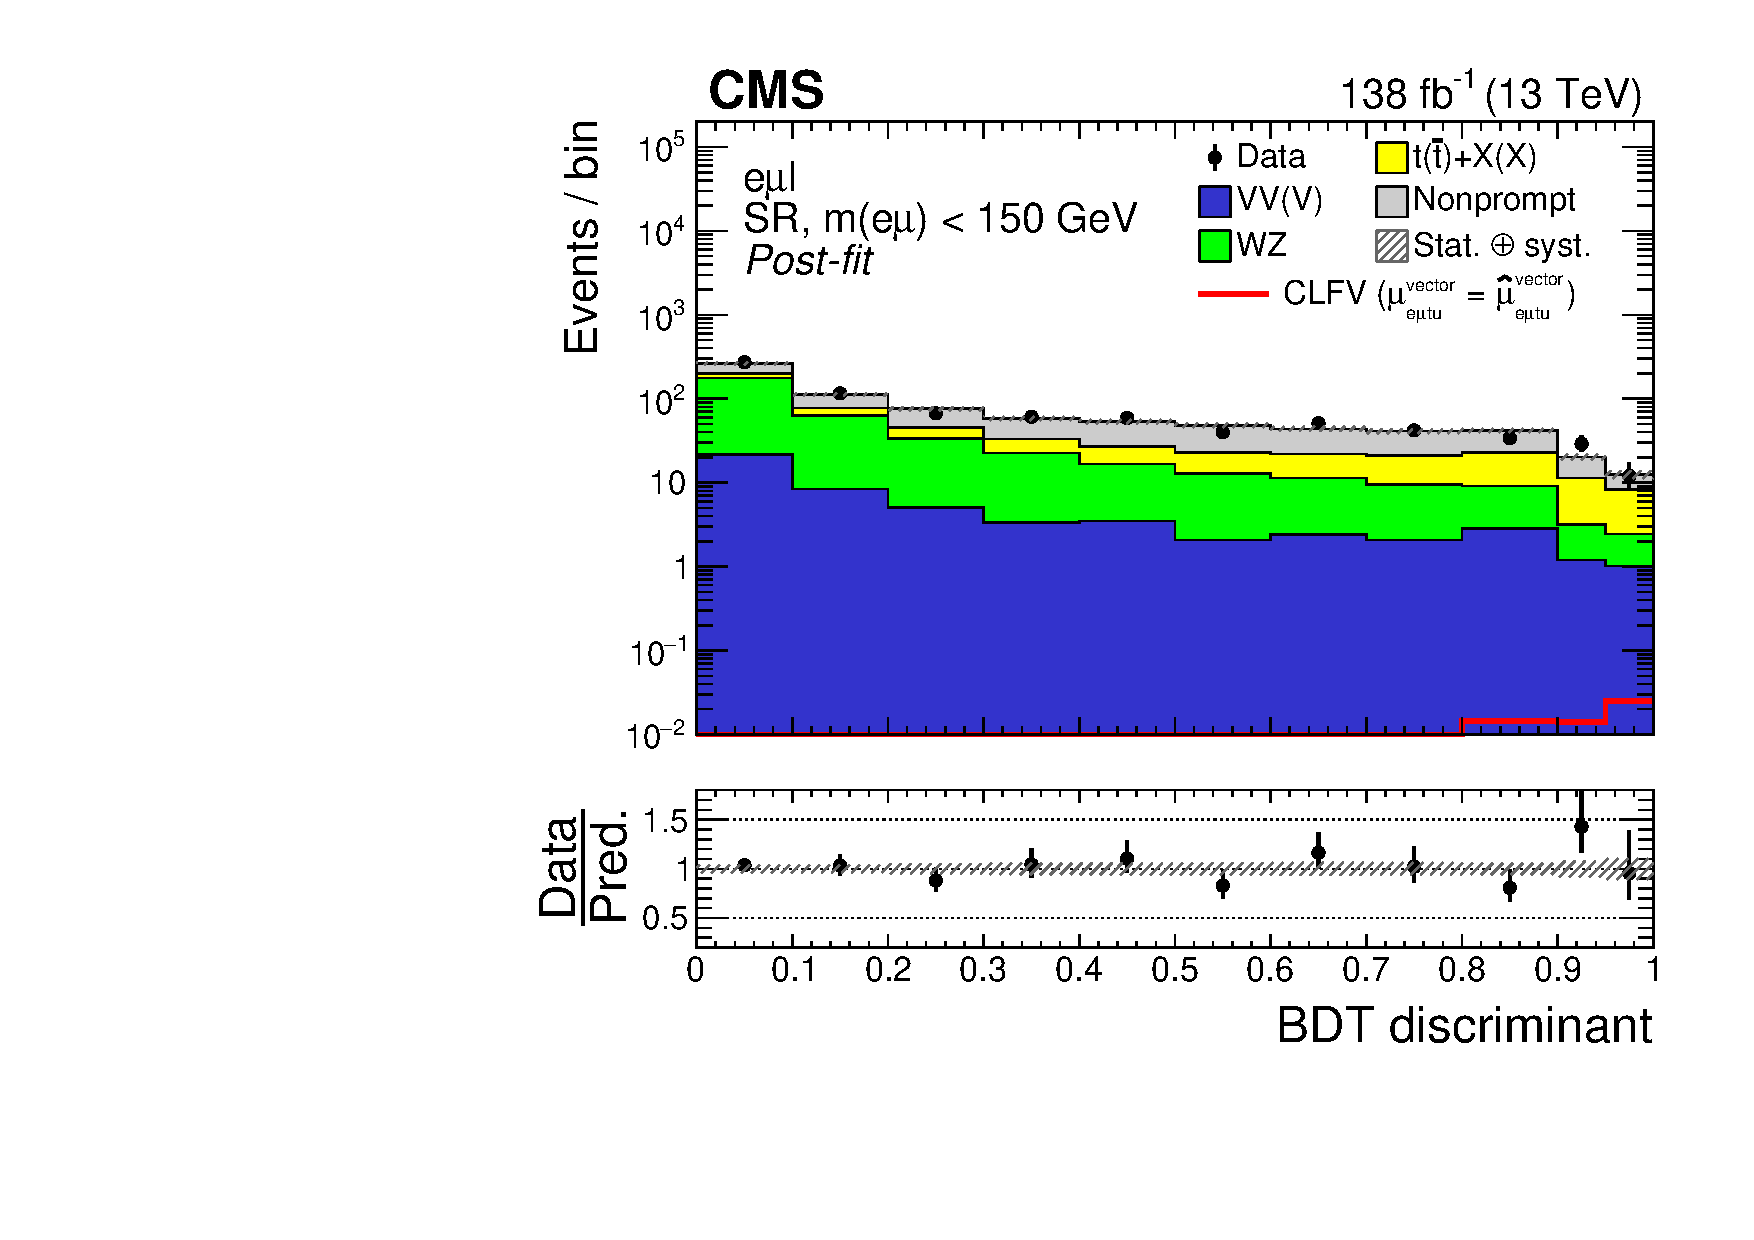
\includegraphics[width=0.48\textwidth]{figures/Part3/Results/BDT_TT_VecU}&
 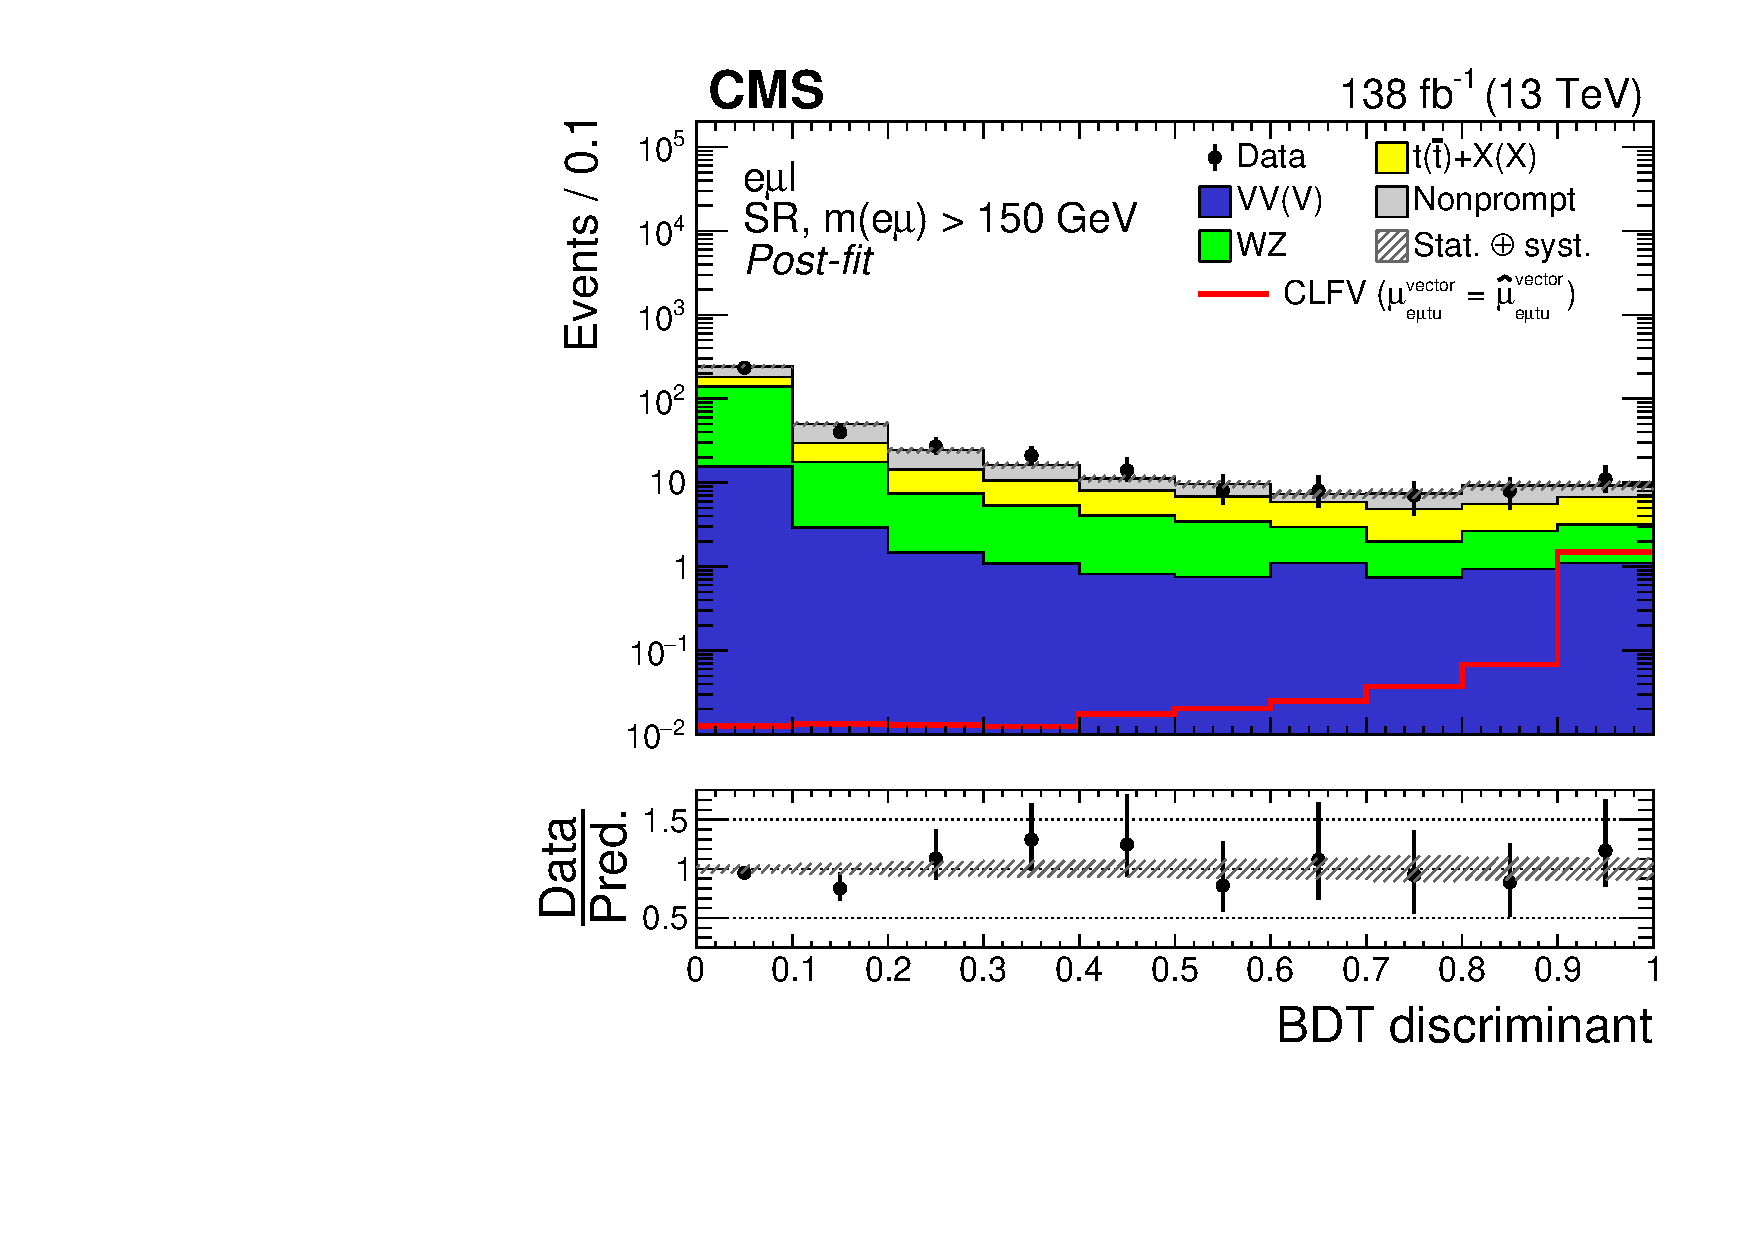
\includegraphics[width=0.48\textwidth]{figures/Part3/Results/BDT_ST_VecU}\\
 \end{tabular}
 \caption{Distributions of the post-fit \ac{BDT} discriminator targeting the \ac{CLFV} top quark decay (left) and production (right) signal. Contributions from the two signal modes (production and decay) are combined within each \ac{SR} and are shown as the solid red line. The post-fit signal strength ($\mu_{\emut{u}}^{\textsf{vector}}=\hat{\mu}_{\emut{u}}^{\textsf{vector}}$) is used to normalise the signal cross sections. The hatched bands indicate post-fit uncertainties (statistical and systematic) for the SM background predictions.}
 \label{fig:bdt_postfit_VecU}
 \end{center}
\end{figure} 

The impacts of the nuisance parameters on the profile likelihood fit are quantified and a representative ranking of the impacts is shown in Figure~\ref{fig:Impact}. In general, the most prominent uncertainties affecting the likelihood fit are the statistical uncertainties that arise from limited sample size. A full collection of nuisance parameter impacts can be found in \autoref{chap:Impact}.

\begin{figure}[tbh!] 
\begin{center}
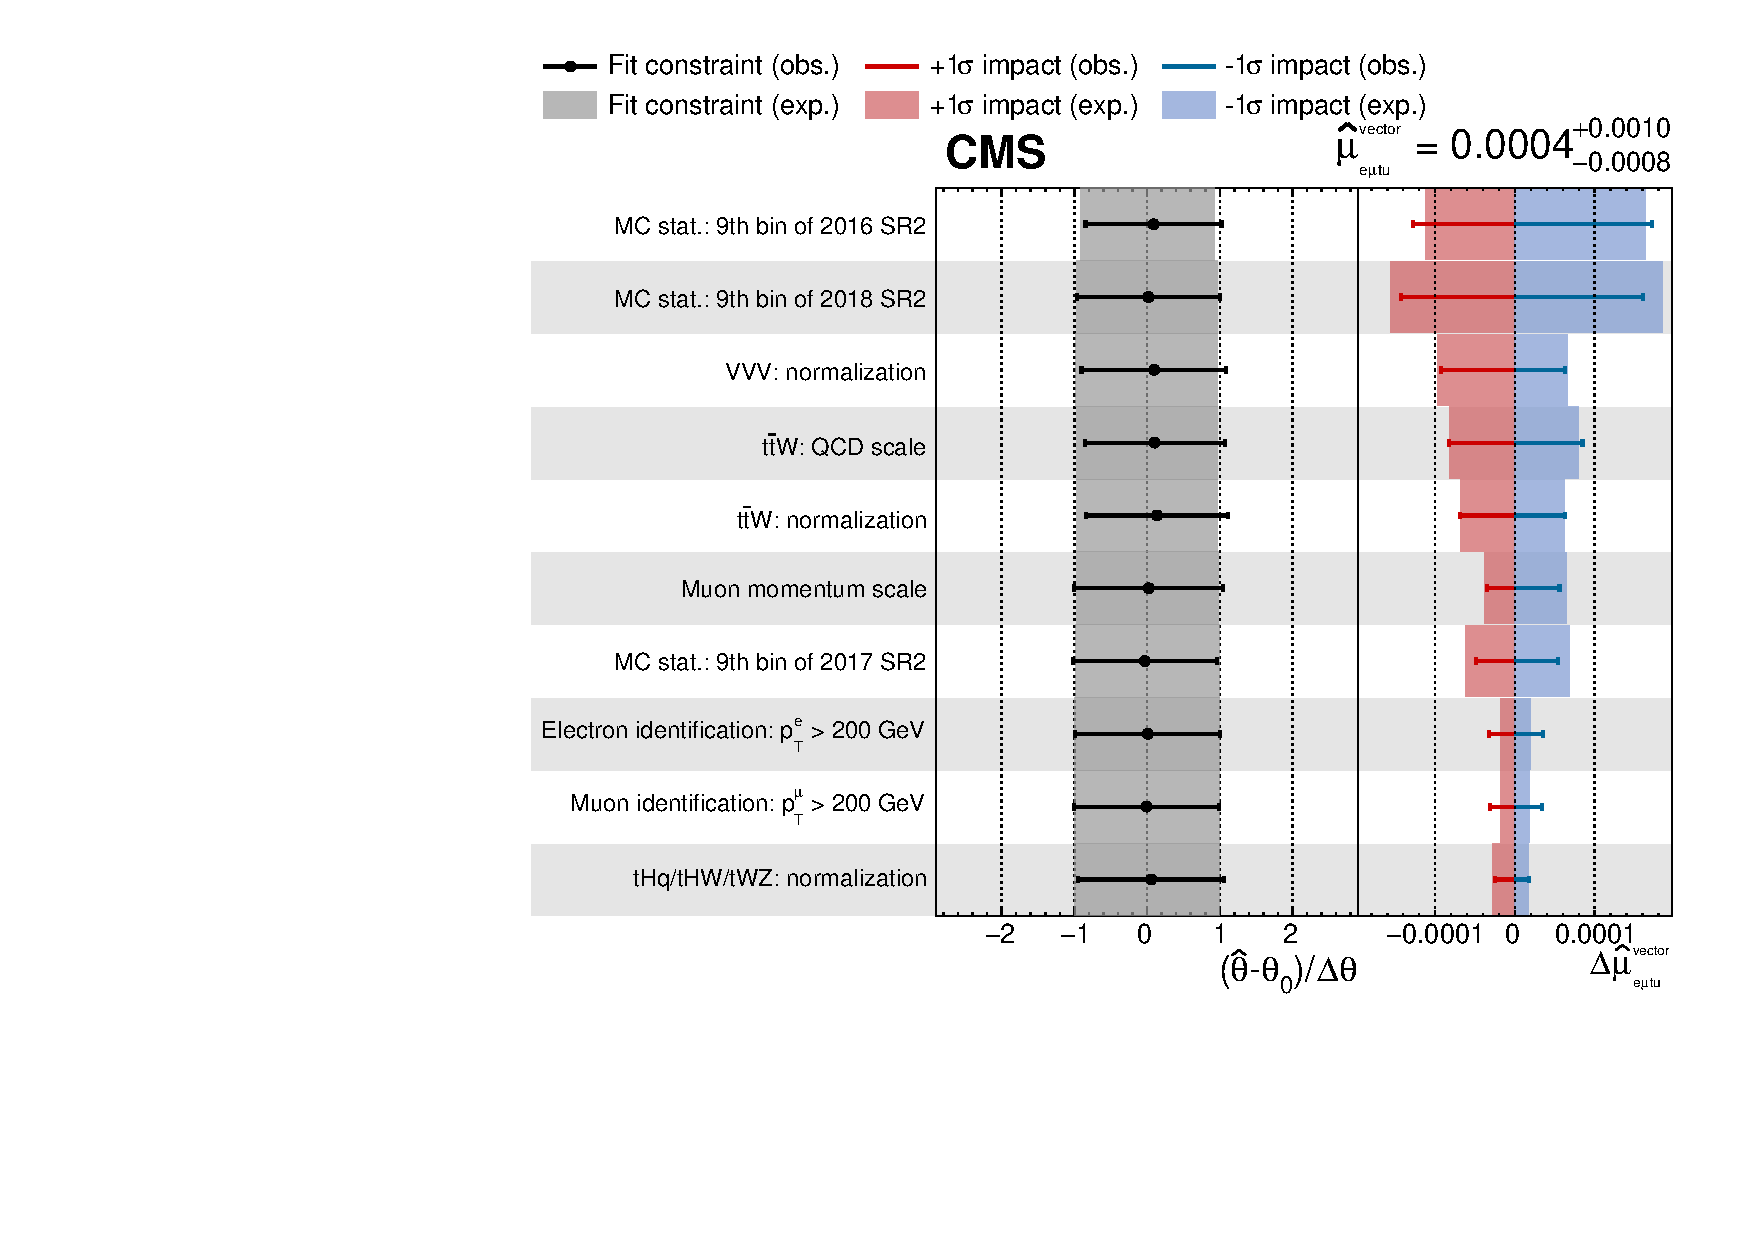
\includegraphics[width=0.9\textwidth]{figures/Part3/Results/Impact_VecU}
 \caption{The nominal value of the observed signal strength $\hat{\mu}$ and its uncertainty is shown in the top right corner. Ranking of the nuisance parameters according to their observed impacts on $\hat{\mu}$ (represented with error bars) is shown in the right panel. Only the 10 nuisance parameters with the largest observed impacts are shown. The expected impacts (represented with red and blue rectangles) are derived using Asimov fits, where data is replaced by a background-only template (i.e. the nominal value of the expected $\hat{\mu}$ is 0). The impact of each nuisance parameter, $\mathrm{\Delta}\hat{\mu}$, is calculated as the difference between the nominal $\hat{\mu}$ and the value of $\hat{\mu}$ when the corresponding nuisance parameter is fixed to $\hat{\theta}\pm\sigma$, where $\hat{\theta}$ ($\sigma$) is its post-fit value (uncertainty). The left panel shows the pulls (represented with black dots) and uncertainties (represented with error bars and grey rectangles) of the nuisance parameters in units of the pre-fit uncertainties. The pulls are calculated as the difference between the nominal and the post-fit values of the nuisance parameters. The ``\ac{SR}2'' quoted in the label corresponds to the top quark production enriched signal region.}
 \label{fig:Impact}
 \end{center}
\end{figure}
%%%%%%%%%%%%%%%%%%%%%%%%%%%%%%%%%%%%%%%%%%%%%%%%%%%%%%%%%%%
%%%%%%%%%%%%%%%%%%%%%%%%%%%%%%%%%%%%%%%%%%%%%%%%%%%%%%%%%%%

\section{Upper Limits}
\label{sec:Limits}

The compatibility between the data and the combined signal plus background expectation under the hypothesized value of the signal strength $\mu$ is quantified by a test statistic that considers the profile likelihood ratio:

\begin{equation}
q(\mu)=-2\ln\frac{\mathcal{L}(\mu,\hat{\theta}_{\mu})}{\mathcal{L}(\hat{\mu},\hat{\theta})}.
\end{equation}

Using the asymptotic modified frequentist CL$_{s}$ method~\cite{Junk:1999kv,Read2002,Cowan:2010js} with the profile likelihood ratio as the test statistic, upper limits are placed on $\mu$ at 95\% \ac{CL}. The one-dimensional upper limits on a given \ac{WC}, $\WC{}{a}/\Lam^2$, are obtained by taking the square root of the corresponding signal strength $\mu_a$ while setting other \acp{WC} to zero. The branching fractions, $\mathcal{B} (\tto{q})$ with q=u or c, are obtained assuming a top quark mass (width) of 172.5 (1.33) GeV in Equation~\ref{eq:4} taken from~\cite{Kile:2008rp}.

The resulting one-dimensional limits are summarized in Table~\ref{tab:limit}. Assuming a linear relationship between $\mathcal{B}(\tto{u})$ and $\mathcal{B}(\tto{c})$ in the case of nonvanishing signals, the two-dimensional limits can be obtained through interpolation and are shown in Figure~\ref{fig:2dlimit}. 

\begin{table}[th]
\sffamily
\centering
\caption{Upper limits at 95\% \ac{CL} on \acp{WC} and the branching fractions. The expected and observed upper limits are shown in regular and bold fonts, respectively. The intervals that contain 68\% of the distribution of the expected upper limits are shown in parentheses.}
\resizebox{0.95\linewidth}{!}{%
\begin{tabular}{cccccc}
\toprule
CLFV & Lorentz & \multicolumn{2}{c}{$\WC{}{\emut{q}}/\mathrm{\Lam}^2~(\TeV^{-2})$} & \multicolumn{2}{c}{$\mathcal{B} (\tto{q}) \times 10^{-6}$} \\
coupling & structure & exp (68\% range) & obs & exp (68\% range) & obs \\
\midrule
\multirow{3}{*}{$\emut{u}$}& tensor & 0.022 (0.018--0.026) & \textbf{0.024} & 0.027 (0.018--0.040) & \textbf{0.032}\\
& vector & 0.044 (0.036--0.054) & \textbf{0.048} & 0.019 (0.013--0.028) & \textbf{0.022}\\
& scalar & 0.093 (0.077--0.114) & \textbf{0.101} & 0.010 (0.007--0.016) & \textbf{0.012}\\
\midrule
\multirow{3}{*}{$\emut{c}$} & tensor & 0.084 (0.069--0.102) & \textbf{0.094} & 0.396 (0.272--0.585) & \textbf{0.498}\\
 & vector & 0.175 (0.145--0.214) & \textbf{0.196} & 0.296 (0.203--0.440) & \textbf{0.369}\\
 & scalar & 0.385 (0.318--0.471) & \textbf{0.424} & 0.178 (0.122--0.266) & \textbf{0.216}\\
 \bottomrule
\end{tabular}
}
\label{tab:limit}
\end{table}

\begin{figure}[tbh!]
 \begin{center}
 \begin{tabular}{cc}
 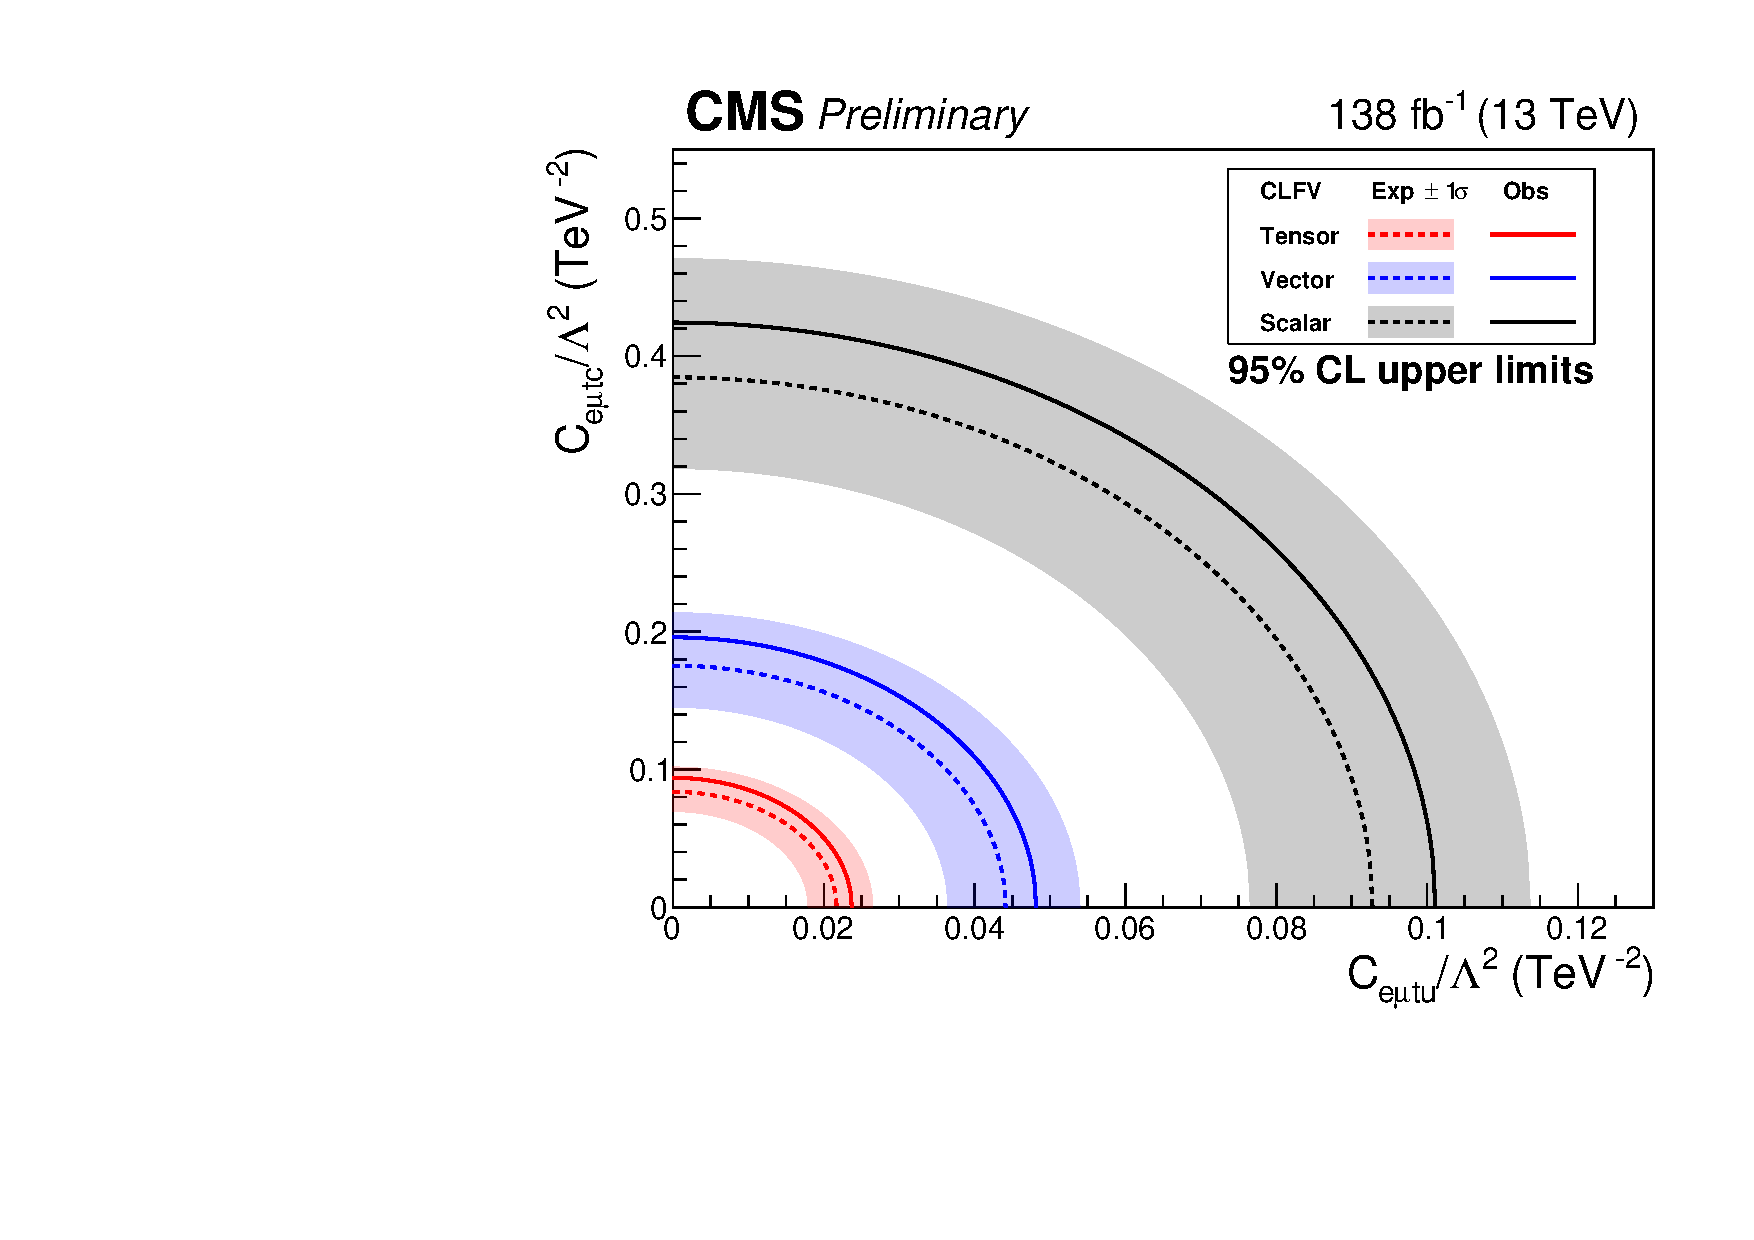
\includegraphics[width=0.48\textwidth]{figures/Part3/Results/Hist2D_WC}&
 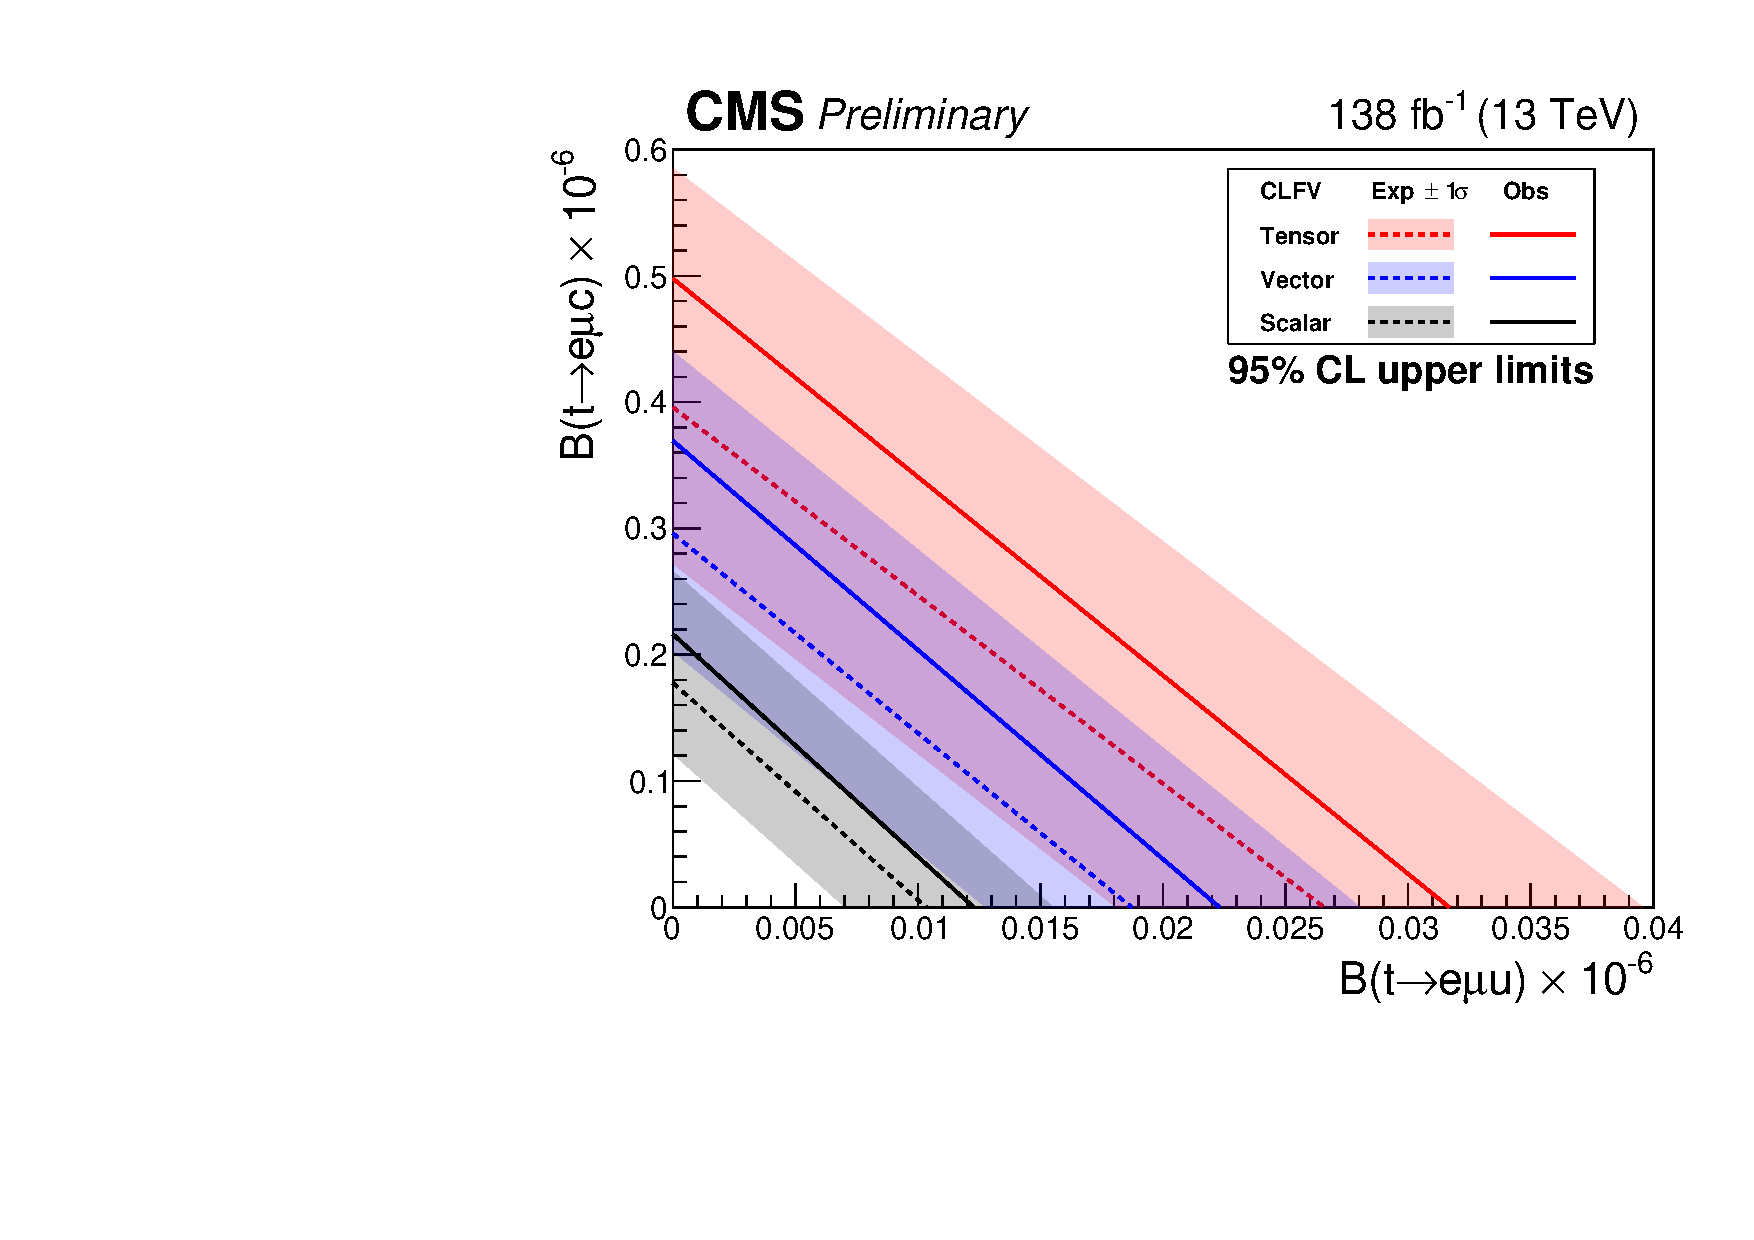
\includegraphics[width=0.48\textwidth]{figures/Part3/Results/Hist2D_BR}\\
 \end{tabular}
 \caption{Two-dimensional 95$\%$ \ac{CL} upper limits on the \acp{WC} (left) and the branching fractions (right). The observed (expected) upper limits for tensor-, vector-, and scalar-like \ac{CLFV} interactions are shown in red, blue, and black solid (dotted) lines, respectively. The shaded bands contain $68\%$ of the distribution of the expected upper limits.}
 \label{fig:2dlimit}
 \end{center}
\end{figure}